%!TEX root = main.tex
\chapter{基于太湖之光的集合全波形反演方法}
\label{ch:基于太湖之光的集合全波形反演方法}
人工地震是由人类通过工业爆破、地下核爆炸、机械撞击等等引起的地震。与天然地震相比,人工地震具有更高的可控性,一般不会对人类经济活动造成巨大的损害。人工地震常用于研究天然地震原因和探测当地矿产资源,是地球物理勘探过程中必不可少的手段。

集合全波形反演方法是地球物理勘探领域非常前沿的地质结构反演方法,与传统的全波形反演方法相比,具备更大的收敛域和更强的抗噪能力,同时也面临着更大的计算挑战。本章通过使用太湖之光超算来设计高效率、高可扩展性的集合全波形反演方法并行模型。

\section{背景知识与算法概述}

\subsection{集合全波形反演方法}

全波形反演方法(full waveform inversion; FWI)于1984年由Tarantola提出,能准确地从人工地震记录中提取大量地下介质信息\cite{tarantola1984inversion,plessix2012full,brossier2009seismic}。该方法通过对比数值模拟合成的地震记录和实际观测的人工地震记录误差,迭代更新模型参数,从而反演地下介质模型\cite{yushu}。然而,由于该方法伴随着巨大的计算开销,直到2010年超级计算机和NVIDIA GPU,Intel MIC等加速器的兴起,为全波形反演方法提供了足够的算力,该方法才逐渐成为研究热点,并为各大石油公司采用。

尽管全波形反演方法在理论上能够很好地反演地下介质模型,但在实际生产中却面临着两大问题。一方面,全波形反演方法需要非常准确的初始速度模型作为输入,否则该算法很容易陷入局部最优\cite{virieux2009overview}。虽然地震记录中的低频信号成分能够降低对初始速度模型的要求,但是在实际生产场景中往往很难捕捉到低频信号\cite{sirgue2006importance}。另一方面全波形反演方法对地震记录数据中的噪音非常敏感,这严重影响了该算法的实际成像效果。

集合全波形反演方法(EnKF)\cite{yushu,he2015ensemble}在传统完全反演\cite{tarantola1982generalized}(total inversion)的基础上,通过使用集合卡尔曼滤波\cite{evensen2003ensemble}中的集合协方差来近似完全反演中协方差算子,这降低了在完全反演中更新协方差算子的计算开销,使之可以在一般的分布式集群中进行计算。然而,由于速度模型中需要更新的参数数量比集合样本数量大2-4个数量级,集合卡尔曼滤波的更新增量受到很大的限制。对此,集合全波形反演方法再次引入了震源编码技术\cite{krebs2009fast}。震源编码技术将所有的震源和地震记录分别进行叠加,每次叠加时不同的震源和地震记录分别使用不同的震源编码,在有利于克服局部收敛的同时\cite{castellanos2014fast},也克服了集合卡尔曼滤波低秩空间的局限性。

均匀介质的声波全波形反演方法可以通过方程\ref{eq:fwi}表示:
\begin{equation}
\label{eq:fwi}
  \min_{m} \phi(m) = \sum_{i=1}^S \rho(\mbox{H}_i(m) - d_{i} ),
\end{equation}
其中$m$表示背景速度模型,$\rho(\cdot)$是一个补偿函数,$d_i=d_1, \ldots, d_S$表示观测数据(实际接收的地震记录),$\mbox{H}_i=\mbox{H}_1, \ldots, \mbox{H}_S$则表示与之相对应的第$i{th}$个正演算子,$S$表示总勘探实验次数(每发射一炮代表一次实验)。这个优化问题通常使用如方程\ref{eq:steepest}形式的迭代算法进行求解:
\begin{equation}
\label{eq:steepest}
m_{k+1} = m_{k} + \alpha_{k}s_k,
\end{equation}
其中$s_k$表示搜索方向,$\alpha_{k}$表示步长。常用的方法包括最速下降法、共轭梯度法等等。

集合全波形反演方法在在每次速度模型更新之后,使用集合卡尔曼滤波对速度模型集合进一步更新,如方程\ref{eq:enkfupdate}所示:
\begin{equation}
\label{eq:enkfupdate}
\left(\mbox{H}\Psi_k^{'}(\mbox{H}(\Psi_k^{'})^T)+D_k^{'}(D_k^{'})^T\right)^{-1}\approx\left((\mbox{H}\Psi_k^{'}+D_k^{'})(\mbox{H}\Psi_k^{'}+D_k^{'})^T\right)^{-1}.
\end{equation}
其中$k$表示第$k$个迭代步,$\Psi_k=(\psi_1^k,\psi_2^k,\ldots,\psi_N^k)$表示有$N$个速度模型样本组成的背景速度场,$D=(d_1^k,d_2^k,\ldots,d_N^k)$表示添加扰动之后的观测数据集合。通过SVD分解,我们有
\begin{equation}
\label{eq:svd}
\mbox{H}\Psi_k^{'}+D_k^{'}=USV,
\end{equation}
其中$U$和$V$是正交矩阵,$S$是对角矩阵。结合方程\ref{eq:enkfupdate}和\ref{eq:svd},我们获得集合更新方程\ref{eq:enkf2}
\begin{equation}
\label{eq:enkf2}
(\Psi_a)_k=\Psi_k+\Psi_k^{'}(\mbox{H}\Psi_k^{'})^TU(SS^T)^{-1}U^T(D_k-H\Psi_k).
\end{equation}
其中$\Psi_a$表示分析速度场。

\subsection{集合全波形反演算法分析}
算法 \ref{alg:enfwicode} 以伪代码的形式描述了集合全波形反演算法。与传统的全波形反演不同,集合全波形反演算法首先需要初始化EnFWI分析步所需要的相关输入,如添加随机扰动后的背景速度场集合、观测数据以及EnFWI分析步所需要的参数(第\ref{ln:enfwiinit}行)。由于背景速度场集合是由同一个初始速度场添加扰动所得,剧烈的扰动会极大改变背景速度场,从而影响全波形反演的成像结果。因此,在进行正式的全波形反演迭代之前,需要执行一次EnFWI分析步计算(第\ref{ln:enfwi1enkf}行),以便为后续的迭代提供一个差异化且较为平滑的初始速度集合。

\begin{algorithm}[ht]
%\scriptsize
%\footnotesize
\small
\caption{集合全波形反演算法伪代码}\label{alg:enfwicode}
\begin{algorithmic}[1]
\State \textbf{//初始化背景速度场集合(vels)、观测数据(obsdata)、EnFWI分析步所需参数(lambdas, ratios)}
\State [vels, obsdata, lambdas, ratios] = init4enkf(); \label{ln:enfwiinit}
\State
\State \textbf{//根据初始速度场进行首次EnFWI分析步计算}
\State enkf\_analyze(vels, obsdata, lambdas, ratios); \label{ln:enfwi1enkf}
\State
\State \textbf{for} (iter = 1; iter < niter; iter++) \{ \textbf{//EnFWI收敛所需运行的总迭代次数} \label{ln:enfwiiter}
\State
\State \quad\quad \textbf{//nsamples为集合样本数目,每一个样本执行独立的震源编码FWI}
\State \quad\quad \textbf{for} (isample = 0; isample < nsamples; isamples++) \{ \label{ln:enfwisample}
\State \quad\quad\quad\quad \textbf{//生成震源编码,并对震源和观测数据进行统一编码}
\State \quad\quad\quad\quad codes = gen\_codec(nshots); \label{ln:enfwicodec}
\State \quad\quad\quad\quad [ensrc, endata, resd, prevgrad, curgrad] = init4essfwi();
\State \quad\quad\quad\quad \textbf{for} (ishot = 0; ishot < nshots; ishots++) \{
\State \quad\quad\quad\quad\quad\quad ensrc += codes[ishot] * srcs[ishot];
\State \quad\quad\quad\quad\quad\quad endata += codes[ishot] * obsdata[ishot];
\State \quad\quad\quad\quad \} \label{ln:enfwicodecend}
\State
\State \quad\quad\quad\quad \textbf{//基于震源编码的地震波正演,计算量最大的函数之一}
\State \quad\quad\quad\quad syndata = forward\_modeling(ensrc, vels[ismaple]); \label{ln:enfwiforward}
\State \quad\quad\quad\quad vsrc = endata - syndata; \label{ln:vsrc}
\State \quad\quad\quad\quad resd += cal\_residual(endata, syndata); \label{ln:resd}
\State
\State \quad\quad\quad\quad \textbf{//基于震源编码的伴随波场反传,计算量最大的函数之一}
\State \quad\quad\quad\quad [vdata, curgrad] = backward\_propagate(vsrc, vels[isamples]); \label{ln:enfwibackward}
\State \quad\quad\quad\quad updatedir = conj\_gradient(prevgrad, curgrad); \textbf{//计算更新梯度方向}
\State \quad\quad\quad\quad swap(prevgrad, curgrad);
\State
\State \quad\quad\quad\quad \textbf{//计算更新步长,计算量最大的函数之一}
\State \quad\quad\quad\quad alpha = cal\_steplen(ensrc, vels[isample], updatedir, resd);
\State \quad\quad\quad\quad update\_vel(alpha, updatedir, vels[isample]); \textbf{//根据梯度和步长更新背景速度场} \label{ln:enfwibackwardend}
\State \quad\quad \} \label{ln:enfwisampleend}
\State
\State \quad\quad \textbf{if} (iter \% enkf\_interval == 0) \{ \textbf{//每隔enkf\_interval迭代步进行EnFWI分析步计算} \label{ln:enfwienkfbegin}
\State \quad\quad\quad\quad enkf\_analyze(vels, lambdas, ratios);
\State \quad\quad \} \label{ln:enfwienkfend}
\State \} \label{ln:enfwiiterend}
\end{algorithmic}
\end{algorithm}

集合全波形反演方法与传统全波形反演的计算流程类似,都是通过迭代算法来求解(第\ref{ln:enfwiiter}到\ref{ln:enfwiiterend}行)。但由于集合全波形反演方法使用集合样本来替代传统全波形反演中的独立样本,集合全波形反演方法需要对集合中的每一个样本独立执行完成的FWI计算(第\ref{ln:enfwisample}到\ref{ln:enfwisampleend}行)。这是集合全波形反演方法引入额外计算开销的最主要原因。集合中的每一个样本都是一个独立的完整全波形反演计算,因此集合全波形反演的计算复杂度与集合的样本数量成线性相关。为了降低计算复杂度,集合全波形反演方法引入了震源编码,在每一个迭代步每一个样本中对所有震源和观测数据进行震源编码(第\ref{ln:enfwicodec}到\ref{ln:enfwicodecend}行),然后对编码后的震源进行线性叠加。未进行震源编码时,全波形反演需要遍历每一炮勘探实验,而进行震源编码之后,不再需要逐炮进行遍历,而是将不同位置的震源根据震源编码同时添加到地震波场中。震源编码技术直接将全波形反演的计算复杂度将为原来的$1/nshots$,其中$nshots$表示炮的数目。这在大规模三维石油勘探中的加速效果非常明显,因为大规模石油勘探中炮击的次数通常为成千上万甚至十万个。值得注意的是,在每个迭代步每个样本的全波形反演中,所有炮击的震源和观测数据使用相同的编码,但在不同迭代步不同样本中,却需要重新生成编码。

随后,以编码后的震源和当前样本速度场作为输入进行地震波正演(forward\_modeling),模拟地震波从震源发射,传播经过不同地下介质,最后到达地震记录接收器的整个过程(时间从$t=0$到$t=nt-1$时刻,第\ref{ln:enfwiforward}行)。由于当前速度场并不是真实的速度场,以此速度场进行正演得到的地震记录成为合成地震记录(syndata)。通过实际观测地震记录和当前合成地震记录,计算可得伴随波场震源(vsrc)和目标函数残差(resd,第\ref{ln:vsrc}行和第\ref{ln:resd}行)。全波形反演的目标则在于最小化目标函数残差,残差越小,代表当前速度模型与真实速度模型越接近。以伴随波场地震和当前速度模型作为输入进行地震波反传(时间从$t=nt-1$到$t=0$时刻),并与对应的正传波场进行相关(correlation)操作,可以求得速度场更新的梯度和步长,用以更新当前速度模型(第\ref{ln:enfwibackward}到\ref{ln:enfwibackwardend}行)。在整个基于震源编码的全波形反演中,计算量最大的三个过程分别是地震波正传、伴随波场反传和计算更新步长。每一个过程都需要对整个波场进行从$t=0:nt-1$或$t=nt-1:0$进行更新。时间步长越短、计算网格分辨率越高或者有限差分算子长度越大都会急剧增大波场更新的计算量,给现代并行计算机带来巨大的挑战。更新波场的过程将在下文详细介绍。对集合中的每一个速度场使用基于震源编码的全波形反演进行更新之后,每隔一定的迭代步,执行集合卡尔曼滤波分析以进一步更新背景速度场集合(第\ref{ln:enfwienkfbegin}到\ref{ln:enfwienkfend}行),然后进入下一个迭代步。

\subsection{集合卡尔曼滤波分析步计算分析}
集合卡尔曼滤波的分析步旨在利用集合替代样本,降低初始速度模型和数据噪音对对算法收敛的影响,提高算法的收敛域。集合全波形反演的额外开销一方面来源于使用集合替代单独样本,在全波形反演中需要为集合中的每个样本单独更新背景速度场。然而,在引入了震源编码之后,震源编码对所有的炮点进行叠加,极大降低了计算复杂度,减轻甚至抵消了集合样本带来的开销。集合全波形反演另一方面的开销则是集合卡尔曼滤波分析步(简称分析步)的计算,虽然并不需要在每个迭代步中都执行分析步计算,但深入分析有利于我们更好地理解集合卡尔曼滤波分析步,并为后续的优化提供可靠的思路。

公式\ref{eq:enkf2}描述了分析速度场的更新方式。结合算法 \ref{alg:enfwicode},我们可以发现如下计算特性:
\begin{itemize}
  \item 分析速度场的更新是所有速度模拟样本的整体更新,而不是像震源编码全波形反演中的每个速度模型独立更新。这里对计算机的内存提出了重大的挑战,尤其是当集合样本数目巨大的时候。
  \item 分析速度场更新的主要计算是大型矩阵和向量代数运算,包括矩阵加法、乘法、转置、求逆等计算密集型的操作,这与太湖之光强大的计算能力十分吻合。
  \item 正演算子$\mbox{H}$,即算法 \ref{alg:enfwicode} 中的forward\_modeling函数仍旧在公式中扮演者重要的作用。通过程序用时解剖(profile)发现,正演算子$\mbox{H}$依旧是EnFWI分析步最耗时的函数,但与算法 \ref{alg:enfwicode}不同,分析步中的正演算子无需设计IO存储,因为分析步中不需要进行地震波反传操作并进行相关(correlation)操作。
\end{itemize}

\begin{table}[ht]
\centering
\caption{集合卡尔曼滤波分析步中不同计算操作耗时百分比。}
\label{tb:enkfprofile}
\begin{tabular}{ccccccc}
\hline
计算操作  & 矩阵加法  & 矩阵乘法  & 矩阵求逆   & 矩阵转置  & 正演算子   & 其他    \\\hline
所占百分比 & 3.2\% & 8.5\% & 17.0\% & 4.3\% & 58.9\% & 8.1\% \\\hline
\end{tabular}
\end{table}
表\ref{tb:enkfprofile}总结了集合卡尔曼滤波分析步中不同计算操作耗时百分比。我们可以发现,优化分析步计算的核心是优化正演算子和矩阵求逆运算。同时,需要同时考虑神威超算系统单节点较小的内存,进行适当的任务划分。

\subsection{地震波波场更新计算分析}
集合全波形反演算法中计算量最大的模块是地震波波场更新,这在算法 \ref{alg:enfwicode} 中体现为$forward\_modeling$、$backward\_propagate$和$cal\_steplen$三个函数,在EnFWI分析步中体现为正演算子$\mbox{H}$。尽管在不同的函数中,更新地震波波场的方式略有不同(有的是正传,有的是反传,有的需要储存波场),但其核心计算都是求解偏微分方程。以$forward\_modeling$为例,离散时间步的波场正演可以用公式来表示:
\begin{equation}
\label{eq:enfwifd}
U_{i+1} = \left[ \Delta U -f(t) \right] v^2 \Delta t^2 + 2 U_{i} - U_{i-1},
\end{equation}
其中 $U_{i-1}$, $U_{i}$ and $U_{i+1}$分别表示上一时间步、当前时间步和下一时间步的波场,$\Delta$表示Laplacian算子,
$f(t)$ 表示震源子波(通常为雷克子波),$v$ 表示速度。算法\ref{alg:acousticfdcode}是均匀介质三维声波正演伪代码,为了方便描述,使用的是基于2阶的有限差分算子\cite{fu2011eliminating}。但是2阶有限差分算子会带来严重的频散,实际生产和研究中,常常使用10阶或者12阶差分算子。



% \begin{algorithm}[ht]
% %\scriptsize
% %\footnotesize
% \small
% \caption{均匀介质三维声波正演伪代码}\label{alg:acousticfdcode}
% \begin{algorithmic}[1]
% \State \textbf{for} ( it = 0; it < nt; it++ ) \{ \label{ln:fdntbegin}
% \State \quad\quad \textbf{for} ( ix = 0; ix < nx; ix++ )
% \State \quad\quad\quad\quad \textbf{for} ( iy = 0; iy < ny; iy++ ) \{
% \State \quad\quad\quad\quad\quad\quad \textbf{for} ( iz = 0; iz < nz; iz++ )\{
% \State \quad\quad\quad\quad\quad\quad\quad\quad  u(it,ix,iy,iz)=2*u(it-1,ix,iy,iz)-u(it-2,ix,iy,iz)+v(ix,iy,iz)*v(ix,iy,iz)*dt*dt*(
% \State \quad\quad\quad\quad\quad\quad\quad\quad\quad\quad\quad\quad\quad\quad\quad                                    u(it-1,ix,iy,iz)*(2/dx/dx+2/dy/dy+2/dz/dz)+
% \State \quad\quad\quad\quad\quad\quad\quad\quad\quad\quad\quad\quad\quad\quad\quad                                    (-u(it-1,ix,iy,ix-1)-u(it-1,ix,iy,ix+1))/dx/dx+
% \State \quad\quad \quad\quad\quad\quad\quad\quad\quad\quad\quad\quad\quad\quad\quad                                    (-u(it-1,ix,iy-1,iz)-u(it-1,ix,iy+1,iz))/dy/dy+
% \State \quad\quad\quad\quad\quad\quad\quad\quad\quad\quad\quad\quad\quad\quad\quad                                    (-u(it-1,iz-1,iy,iz)-u(it-1,iz+1,iy,iz))/dz/dz);
% \State
% \State \quad\quad\quad\quad\quad\quad\quad\quad \textbf{if} ( is\_boundary(ix, iy, iz) ) \textbf{//吸收边界处理} \label{ln:fdboundary}
% \State \quad\quad\quad\quad\quad\quad\quad\quad\quad\quad\quad    apply\_absorb\_boundary\_condition(u);
% \State \quad\quad\quad\quad\quad\quad                \} \label{ln:fdntend}
% \State \quad\quad\quad\quad\quad\quad \textbf{if} (is\_record\_seismo) \textbf{//输出合成地震记录}
% \State \quad\quad\quad\quad\quad\quad\quad\quad save\_seismo(u(it, ix, iy, :);
% \State \quad\quad\quad\quad \}
% \State
% \State \quad\quad \textbf{if} ( is\_record\_wavefield ) \textbf{//输出波场快照}
% \State \quad\quad\quad\quad output\_wavefield(u(it, :, :, :));
% \State
% \State \quad\quad \textbf{for} ( is = 0; is < ns; is++ ) \textbf{//在正传波场中添加震源信号}
% \State \quad\quad\quad\quad u(it, src[is].x, src[is].y, src[is].z) += wavelet(is, it);
% \State \}
% \end{algorithmic}
% \end{algorithm}

算法\ref{alg:acousticfdcode}仅描述了在一个速度模型样本,单个震源或者震源编码情况下的地震波正演。在传统的多震源正演和全波形反演中,不同震源之间是相互独立的,可以完全使用不同的节点分别对不同的震源进行地震波模拟,相互之间没有通信开销(全波形反演算法中有少量的通信)。因此,提升正演算子的性能只需要关注单个样本、单个震源下的地震波传播模拟即可。地震波正演过程中,核心计算是在$t=0$到$t=n-1$时刻不停往波场中注射震源激励信号、更新波场(第\ref{ln:fdntbegin}到\ref{ln:fdntend}行),并根据需要输出合成地震记录或者正传波场:
\begin{itemize}
  \item 在$forward\_modeling$函数中,需要同时输出合成地震记录和正传波场。合成地震记录用以计算目标函数残差,正传波场用以在$backward\_propagate$函数中与伴随波场进行相关(correlation)操作。
  \item 在$backward\_propagate$函数中,合成地震记录和正传波场都无需输出,但需要读取$forward\_modeling$中的正传波场。
  \item 在$cal\_steplen$函数中,只需要输出合成地震记录,用以确定更新步长。
\end{itemize}

在生产环境中,虽然我们在一定的范围内进行人工地震石油勘探,但地震波的传播并不会限定在特定范围,而是无穷无尽向四面八方传播。而在数值模拟过程中,由于人为规定了模拟的区域,地震波到达规定区域的边界时会进行反弹,这便于实际情况不符。因此,在数值模拟中,我们常在模拟区域的边界处添加吸收边界条件(absorb boundary condition,第\ref{ln:fdboundary}到\ref{ln:fdntend}行),消除地震波在边界处的反射现象。



正演算法在神威超算上的并行优化挑战主要有两个。第一个是有限差分算子需要较高的数据重用与申威处理器从核有限的LDM空间之间的挑战。算法\ref{alg:acousticfdcode}使用的是如图\ref{fig:stencilstruct}(a)中的7点星形stencil算子。对于每一个中心点进行更新时,需要访问中心点的上下左右前后方向各1个点。面对更复杂的stencil时,如图\ref{fig:stencilstruct}中的19点或者27点结构,则需要访问更多的邻接格点来更新中心格点。在集合全波形反演算法中,使用的是31点的10阶星形stencil。每一个点都需要复用5次。尽管每个邻接格点距离中心点很“近”,但在物理内存的连续存储中,不同的邻接格点却相距甚远,分别相距若干行、若干列甚至若干平面。在Intel CPU架构下直接进行访问时,会出现大量的cache miss,从而反复从内存中加载数据,计算效率非常低下。在Intel CPU架构中,高效的stencil运算操作需要充分利用L1、L2高速缓存,尽可能在一个点未完全访问完毕后锁定在cache中\cite{datta2008stencil,datta2009optimization,sellappa2004cache}。GPU架构下的多层级内存结构非常适合stencil运算,一方面来自于GPU高效的内存带宽,另一方面开发者手动可控的共享内存(shared memory)也为stencil的优化提供了巨大的便利\cite{meng2009performance,nguyen20103,micikevicius20093d}。对于神威超算系统而言,每个从核虽然具备类似GPU共享内存的LDM高速缓存,但是每个从核的LDM大小只有64KB,无法装载大量格点。此外,GPU显存的带宽显著高于神威超算的内存带宽,而stencil运算又是典型的访存受限问题,这也给stencil的优化带来巨大的挑战。

另一个挑战来源于正演算法的流程本身。波场更新的每一步都需要注射震源,在震源编码叠加之后,震源的位置分布不连续,在三维勘探中,震源分布在水平面。如果把添加震源的操作放在申威处理器的主核完成,则效率低下,如果交给从核计算,由于DMA加载数据不连续且块大小非常小,DMA效率也很低下。另一方面,在每个申威核组只有8GB内存的情况下,$forward\_modeling$函数无法将所有正演波场存储在内存中,必须通过IO输出到磁盘中。但输出波场到磁盘中的也面临两个挑战。首先,在三维正演模拟中,每个波场的大小约为0.5-4GB(根据区域划分确定),每次模拟需要执行$10^4$值$10^7$个时间步,如果将所有的波场输出到磁盘,磁盘将面临500GB-10PB的空间压力,这并不是一般的磁盘阵列能够承受的。其次,神威超算采用的是网络文件系统,每个节点并没有独立的本地磁盘,当进行成千上万甚至十万进程大规模IO输出是,如果均衡分配IO代理,调度IO进程则显得尤为重要。


\subsection{设计与优化思路}

针对上述集合全波形反演的诸多问题与挑战,结合太湖之光超算系统结构特性,我们从以下几方面考虑高效的并行设计优化策略。

合理的并行任务划分机制。神威超算系统的共有40960个计算节点,而排名第二的天河2号仅有16000个计算节点\cite{tianhe-2}。然而神威系统单节点主频只有1.45GHz,而天河2号则为2.2GHz。良好的并行任务划分策略能够充分利用神威超算的众多节点优势,同时克服单节点内存不足的劣势。集合全波形反演应用中,我们设计了高效的多层级并行任务划分机制,分别从集合样本、三维模型区域分解、单核组从核内部分块等三方面将集合全波形反演算法高效率扩展多8192个神威超算核组。

高效的LDM缓存数据重用。 高效利用神威从核LDM缓存是提升单节点stencil运算的重点。对于类stencil等访存受限算法,优化的核心是提高数据复用率,降低内存访问。神威从核LDM缓存是数据复用的最佳场所,因此我们尽可能让格点停留在有限的LDM中,直到对该格点的所有访问结束。从核通过DMA将数据从主存传输到LDM中,这是stencil计算的最主要开销。DMA的传输效率受每次DMA传输数据的块大小影响,我们通过数学建模,推导出在不同情况下最优的DMA传输配置。此外,为了进一步提高LDM的有效利用率,降低重复的DMA数据传输,我们还提出了函数融合、寄存器通信、从核ID重映射等优化方案。

随机边界处理与数据压缩。在$forward\_modeling$函数中,存储正演波场的目的是为了与在$backward\_propagate$函数中反传的地震波场做相关(correlation)操作,求解更新速度模型的梯度。在密集的计算流程中频繁执行IO操作极大地降低了整体计算效率。一种可行的方法是根据声波方程的可逆性,只存储$t=n-1$和$t=n-2$时刻的波场,并按照声波方程求解$t=n-3$到$t=0$时刻的波场。与前者相比,后者用重复计算换取IO开销,这通常能获得更高的效率。然而,声波方程的可逆性无法处理边界问题。后者方法仍然需要存储不同时间步波场的边界,并在反传时读取覆盖已有的边界,以保证与伴随波场的正确相关。为了进一步降低对IO的依赖,以更多的计算替代IO开销,更充分发挥神威超算的计算性能,本研究使用随机边界处理方法,该方法使用随机数消除了震源波场与伴随波场的耦合性,以可接受的边界吸收精度抵消了震源波场的边界存储,提升了整体计算性能。此外,我们还是用了LZ4算法对合成地震记录进行压缩,缩小合成地震记录的体积,节约IO带宽的同时缩短了IO时间。






% section 基于集合样本的多层级并行任务分解 (end)

\section{面向stencil运算的LDM高效数据复用} % (fold)
\label{sec:面向stencil运算的ldm高效数据复用}



\subsection{三维划分下最小DMA数据传输推导} % (fold)
\label{sub:三维划分下最小DMA数据传输推导}

% subsection 三维划分下最小DMA数据传输推导(end)






% section 面向stencil运算的ldm高效数据复用 (end)

\section{随机边界条件与合成地震记录压缩} % (fold)
\label{sec:随机边界条件与合成地震记录压缩}

地震波震源波场的存储或地震波边界波场的储存是地震波伴随时进行相关(correlation)操作必不可少的的条件。当运行大规模集合全波形反演时,由于神威超算没有本地盘,地震波场的存储成为了程序整体效率的瓶颈之一。本小节将应用随机边界条件替代地震波场的存储,提升程序运行的整体效率。

在震源波场和伴随波场的相关操作中,由于声波方程的可逆性,只有震源波场和伴随波场中相互耦合的数据会对相关的结果(成像)造成影响。随机边界的原理与吸收边界不同,它并不会在边界处吸收波场的能量,而是在边界处添加随机速度层。当地震波到达边界时发生随机散射,以此来降低伴随波场的耦合性,减少人工边界造成的成像影响。随机边界处的散射效果越好,震源波场和伴随波场的相关性就越低。

算法\ref{alg:randomboundary}是随机边界算法的伪代码。边界的处理在遍历完成波场的内部,往往发生在边界内波场更新完毕之后。第\ref{ln:randbegin}到第\ref{ln:randend}行表示不断寻找满足稳定性条件的随机散射点,然后替换已有的边界速度,随后进入下一个边界点处理。

\begin{algorithm}[ht]
%\scriptsize
%\footnotesize
\small
\caption{随机边界算法伪代码}\label{alg:randomboundary}
\begin{algorithmic}[1]
\State \textbf{for} ( ix = 0; ix < nx; ix++ )
\State \quad\quad \textbf{for} ( iy = 0; iy < ny; iy++ )
\State \quad\quad\quad\quad \textbf{for} ( iz = 0; iz < nz; iz++ )\{
\State \quad\quad\quad\quad\quad\quad \textbf{// 其他计算处理}
\State \quad\quad\quad\quad\quad\quad \textbf{if} (is\_boundary(ix, iy, iz)) \{ \textbf{// 边界情况处理}
\State \quad\quad\quad\quad\quad\quad\quad\quad \textbf{while} (true) \{ \label{ln:randbegin}
\State \quad\quad\quad\quad\quad\quad\quad\quad\quad\quad r = rand();
\State \quad\quad\quad\quad\quad\quad\quad\quad\quad\quad vv = v(ix, iy, iz) + r * d; \textbf{// 构造散射条件,d为边界厚度}
\State \quad\quad\quad\quad\quad\quad\quad\quad\quad\quad \textbf{if} (is\_stable(vv)) \{
\State \quad\quad\quad\quad\quad\quad\quad\quad\quad\quad\quad\quad v(ix, iy, iz) = vv; \textbf{// 散射点替换已有速度}
\State \quad\quad\quad\quad\quad\quad\quad\quad\quad\quad\quad\quad break;
\State \quad\quad\quad\quad\quad\quad\quad\quad\quad\quad \}
\State \quad\quad\quad\quad\quad\quad\quad\quad \} \label{ln:randend}
\State \quad\quad\quad\quad\quad\quad \}
\State \quad\quad\quad\quad \}
\end{algorithmic}
\end{algorithm}

另一个耗时较大的模块是合成地震记录的文件输出。精确模型的合成地震记录场作为观测合成地震记录用于全波形反演或逆时偏移算法,因此这部分输入无法省略。合成地震记录输出具备以下特点:
\begin{itemize}
  \item 输出体量大:对于中等规模的地震模拟,合成地震记录文件的大小约为10GB到1T;
  \item 每次输出等量数据:程序中并不存储所有合成地震记录(内存不足),往往输出每一个接收器或每个平面的所有时间步收集的数据;
  \item 大量数据为0:接收器距离震源的距离不一,在震源的直达波到达接收器前,接收器接收不到地震波直达或反射信号。
\end{itemize}
综合以上特点,我们使用LZ4算法对合成地震记录进行压缩,有效地减小了合成地震记录的文件规模。

% section 随机边界条件与合成地震记录压缩 (end)

\section{其他优化方法} % (fold)
\label{sec:其他优化方法}



% section 其他优化方法 (end)

\section{实验结果与分析} % (fold)
\label{sec:实验结果与分析}

\subsection{基于神威超算的并行实现}

采用上文介绍的多层级划分方案、最小DMA数据传输总量推导、寄存器通信等等优化策略,我们在太湖之光上实现了二维和三维的集合全波形反演应用的主核和从核版本。并基于集合样本和波场区域分解将应用扩展到了8192个进程,充分地利用了太湖之光的大规模计算能力。

神威超算的主核的主频低、逻辑与计算处理能力较弱,从核又无法为主核分担,无法执行通信、IO等操作,性能的瓶颈集中在主核中。因此,本研究尽可能将所有函数移植到从核中,只让主核处理必要的调度、通信、IO等操作。

本文采用了OpenACC和Athread两种并行实现方式,针对不同的函数采取最优的实现。OpenACC具有编程易用性强、开发时间短、可维护性高等优势,集合全波形反演算法中大量的基本向量/矩阵运算如向量/矩阵加法、矩阵/乘法等简单的函数采用了OpenACC并行方法实现。而计算行为较为复杂的函数都采用控制粒度更细的Athread并行方法实现。按照分配线程、DMA数据读取、LDM中数据计算,DMA数据写出流程进行编程实现和性能优化。

在单节点性能取得极致之后我们开始进行多节点并行扩展。本研究中单个样本的速度模型的最大网格大小为$920\times 300 \times 500$,我们按照$8\times 2 \times 4$进行划分以获得接近立方体的子网格,每个子网格的大小为$115\times150\times125$。每个子网格分配给一个MPI进程。集合的样本数目为128个,总MPI进程数到到8192。

由于本实验反演的是中小规模的地质模型,因此并未将太湖之光的所有计算资源充分利用。但本研究为太湖之光定制的集合全波形反演应用是面向大规模三维反演成像设计的,因此充分具备反演大规模模型的能力。

\subsection{性能优化结果}

本小节展示在太湖之光超算平台上针对集合全波形反演应用进行性能优化的结果。图\ref{fig:集合全波形反演算法核心函数从核优化加速比}表示集合全波形反演算法核心函数从核优化加速比。\emph{Intel单核}表示该函数在Intel Xeon E5-2697v2(主频为2.7GHz)机器的性能。为了进行更加公平的对比,Intel平台的结果也是经过深度优化的,包括向量化、缓存分化快(cache blocking)、循环展开等等。\emph{主核}表示神威主核的性能,这是作为比较的基准。\emph{64从核}表示使用64个从核进行深度优化后的性能。

从图\ref{fig:集合全波形反演算法核心函数从核优化加速比}可知,Intel单核性能普遍为神威主核性能的4倍,其中重要的原因是Intel的主频较高。经过64个从核优化之后,不同函数的加速比分布在$6.5\times$至$32.3\times$。性能最好的$fd2t10s$函数取得了32.3倍的加速。这个函数是空间10阶、时间2阶的有限差分运算的核心函数,同时也是$fwd\_prop$、$back\_prop$、$cal\_steplen$等函数的核心子函数。因此,在深度优化$fd2t10s$之后,$fwd\_prop$、$back\_prop$、$cal\_steplen$等函数也相应获得了21至28倍的性能提升。

使用64个从核加速仅获得不足30倍的加速比,效率不足50\%,这似乎不是令人激动的数字。然而当我们对有限差分算法进行深入分析之后发现,空间为10阶的中心stencil运算是严重的访存受限问题,性能的提升取决于数据的复用以及对访存带宽的利用率。经过我们的细致优化(包括多层级数据划分、数组融合、寄存器通信,从核ID重映射、内存字节对齐等等),$fd2t10s$函数的DMAD带宽效率达到了26GB/s,达到了神威单核组的访存峰值带宽的74\%,在有限的LDM中,这几乎达到了有效访存带宽的极致。

$pack$函数是进行MPI通信前,将波场边界的不连续数据拷贝到连续的数组中以便组成大块的连续消息,$unpack$函数则是对应的逆向过程。这两个函数的核心是进行内存复制,主要的瓶颈是内存带宽,因此优化这两个函数仅获得7倍左右的性能提升。

\begin{figure}[ht]
\centering
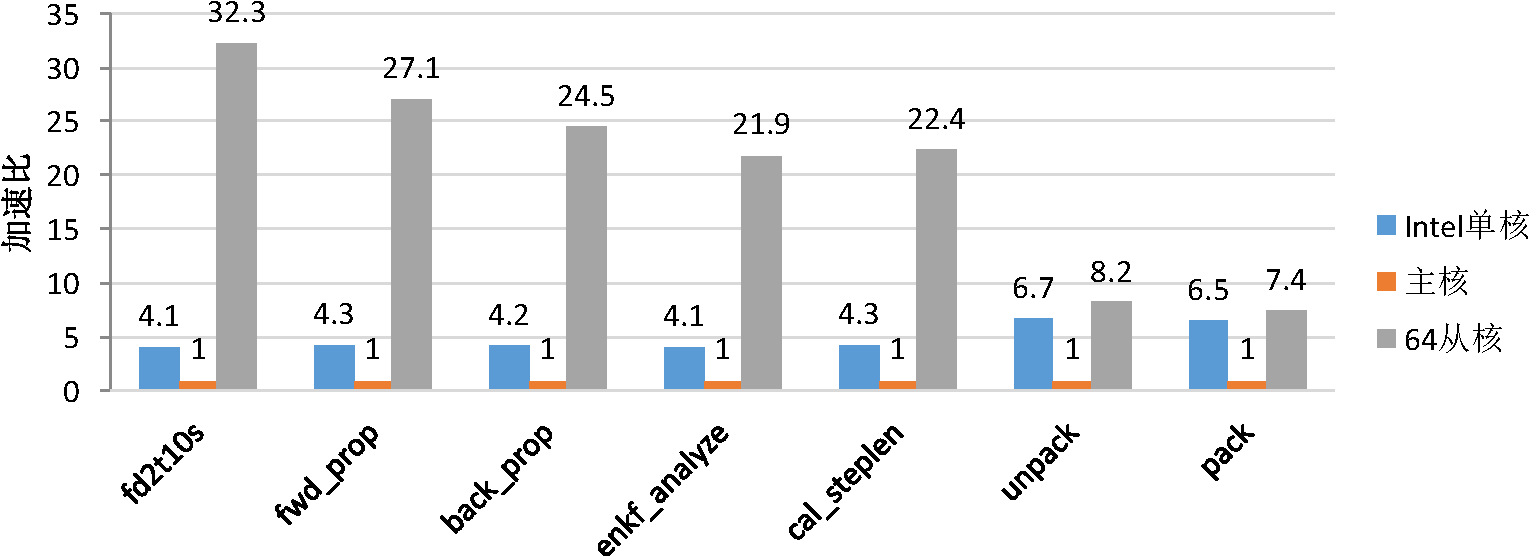
\includegraphics[width=0.9\columnwidth]{enfwi不同函数优化加速比-crop.pdf}
\caption{集合全波形反演算法核心函数从核优化加速比。}
\label{fig:集合全波形反演算法核心函数从核优化加速比}
\end{figure}



\subsection{数值实验模拟}
本小节使用数值实验模拟,比较传统全波形反演算法、震源编码全波形反演方法和集合全波形反演算法在叫不精确的初始速度模型以及有噪音的数据下的收敛情况。验证集合全波形反演方法有较大的收敛域和较小的数据噪音敏感度。

本算例中,我们对Marmousi模型进行反演,Marmousi模型是典型的二维全波形反演模型,为了使用该模型进行三维集合全波形反演,我们人为地将二维平面扩展成三维,扩展后的模型的大小为$9.2km\times 3.0km \times 5km$,空间步长为$10m$,网格的大小为$920\times 300 \times 500$。我们将震源放置在深度为$10m$的平面,在平面上每个$100m$放置一个震源,震源函数为
\begin{equation}
  f(t)=\sin(2\pi f_0t)\cdot e^{-4\pi^2f_0^2t^2/16}
\end{equation}
其中主频$f_0$为10Hz,$t$为时间。地震记录接收器(检波器)同样铺放在深度为$10m$的平面,且每个$10m$放置一个检波器,检波器铺满整个平面网格。正演的时长为$3s$。伪三维Marmousi模型正演反演数值模拟参数如表\ref{tb:伪三维Marmousi模型正演反演数值模拟参数}所示。

\begin{table}[ht]
\centering
\caption{伪三维Marmousi模型正演反演数值模拟参数}
\label{tb:伪三维Marmousi模型正演反演数值模拟参数}
\begin{tabular}{cccccc}
\hline
参数 & 反演范围($km^3$) & 分辨率 & 网格大小        & 震源频率 & 正演时长 \\\hline
配置 & 9.2*3.0*5     & 10m   & 920*300*500   & 10Hz    & 3s  \\\hline
\end{tabular}
\end{table}

Marmousi的精确速度模型如图\ref{fig:Marmousi精确模型}所示。我们使用精确速度模型进行正演得到实际观测地震记录,然后我们在精确速度模型的慢度域进行模糊化处理,平滑的窗口的大小为为$1.8km\times 0.5km$,平滑后的模型如图\ref{fig:Marmousi模型慢域平滑后的初始模型}所示。平滑后的模型(即初始速度模型)和实际观测地震记录作为集合全波形反演的输入,目标是经过300次迭代步之后,将初速速度模型反演逼近得到如图\ref{fig:Marmousi精确模型}所示的精确速度模型。

\begin{figure}[ht]
    \centering
    \begin{subfigure}[b]{0.5\textwidth}
        \centering
        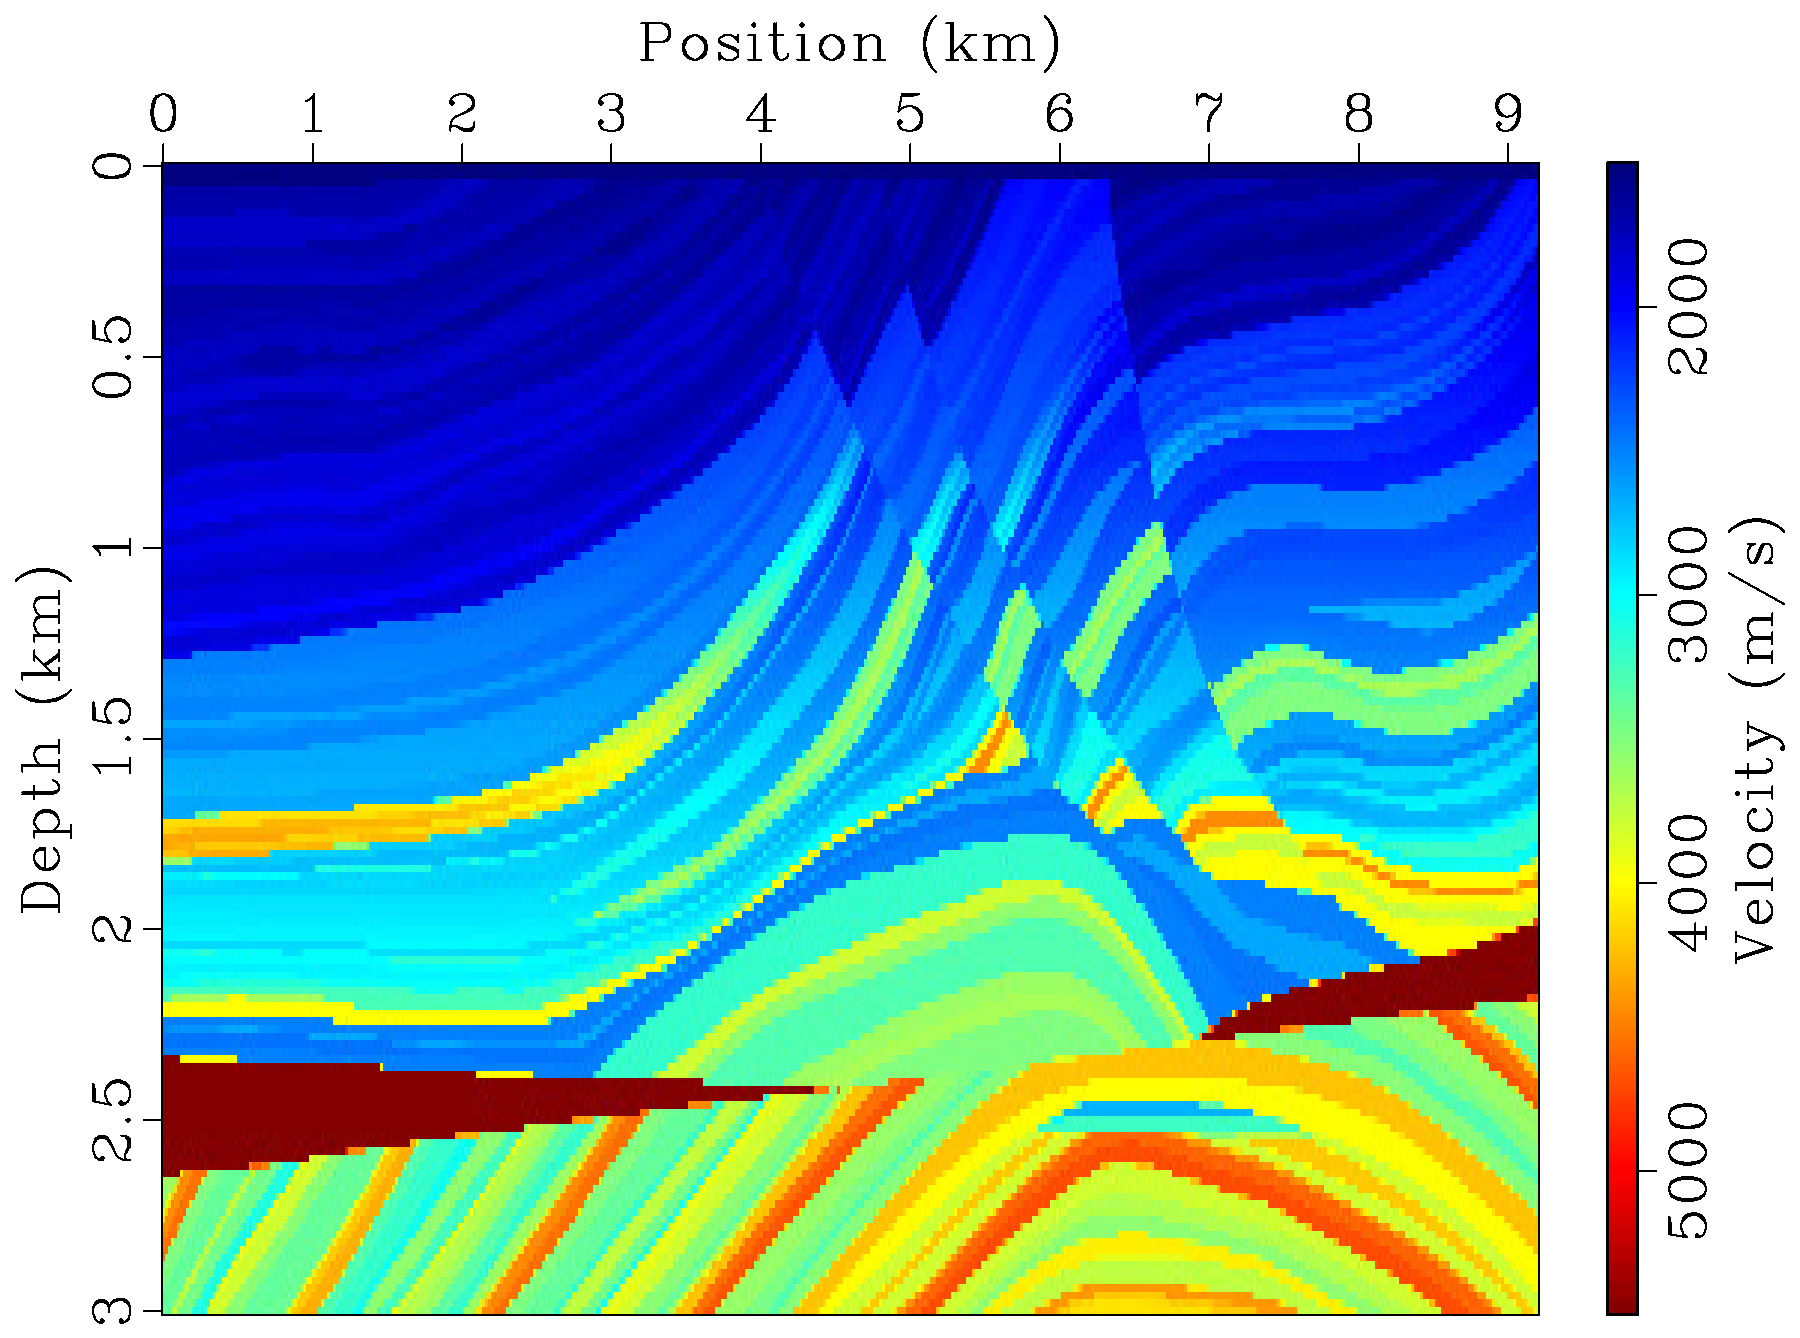
\includegraphics[height=2.1in]{marmvel.pdf}
        \caption{Marmousi精确模型。}
        \label{fig:Marmousi精确模型}
    \end{subfigure}%
    ~
    \begin{subfigure}[b]{0.5\textwidth}
        \centering
        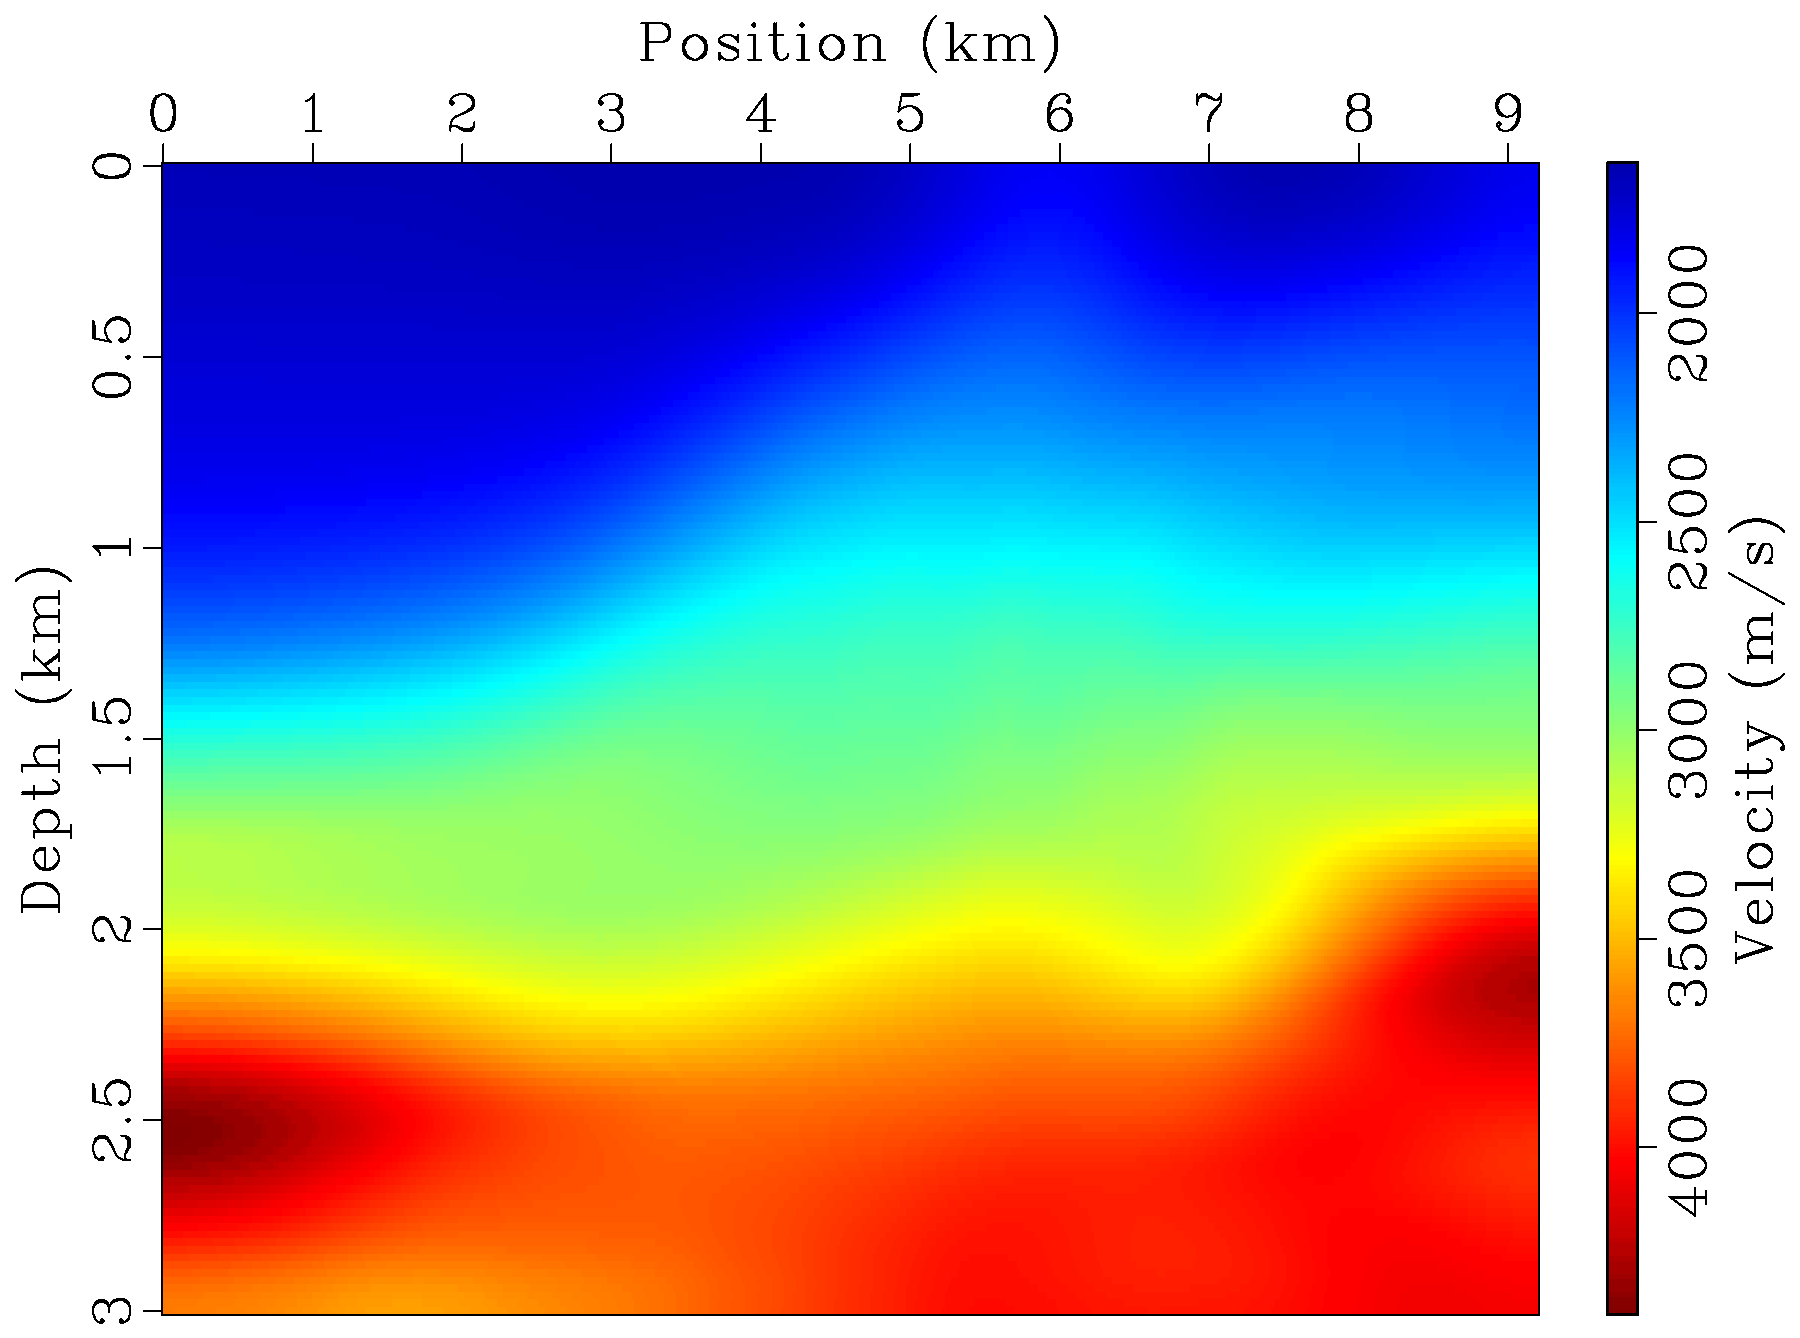
\includegraphics[height=2.1in]{marmvel_smoothed.pdf}
        \caption{Marmousi模型慢域平滑后的初始模型。}
        \label{fig:Marmousi模型慢域平滑后的初始模型}
    \end{subfigure}
    \caption{Marmousi精确模型和平滑后的初始模型}
    \label{fig:Marmousi精确模型和平滑后的初始模型}
\end{figure}


\begin{figure}[ht]
    \centering
    \begin{subfigure}[b]{0.5\textwidth}
        \centering
        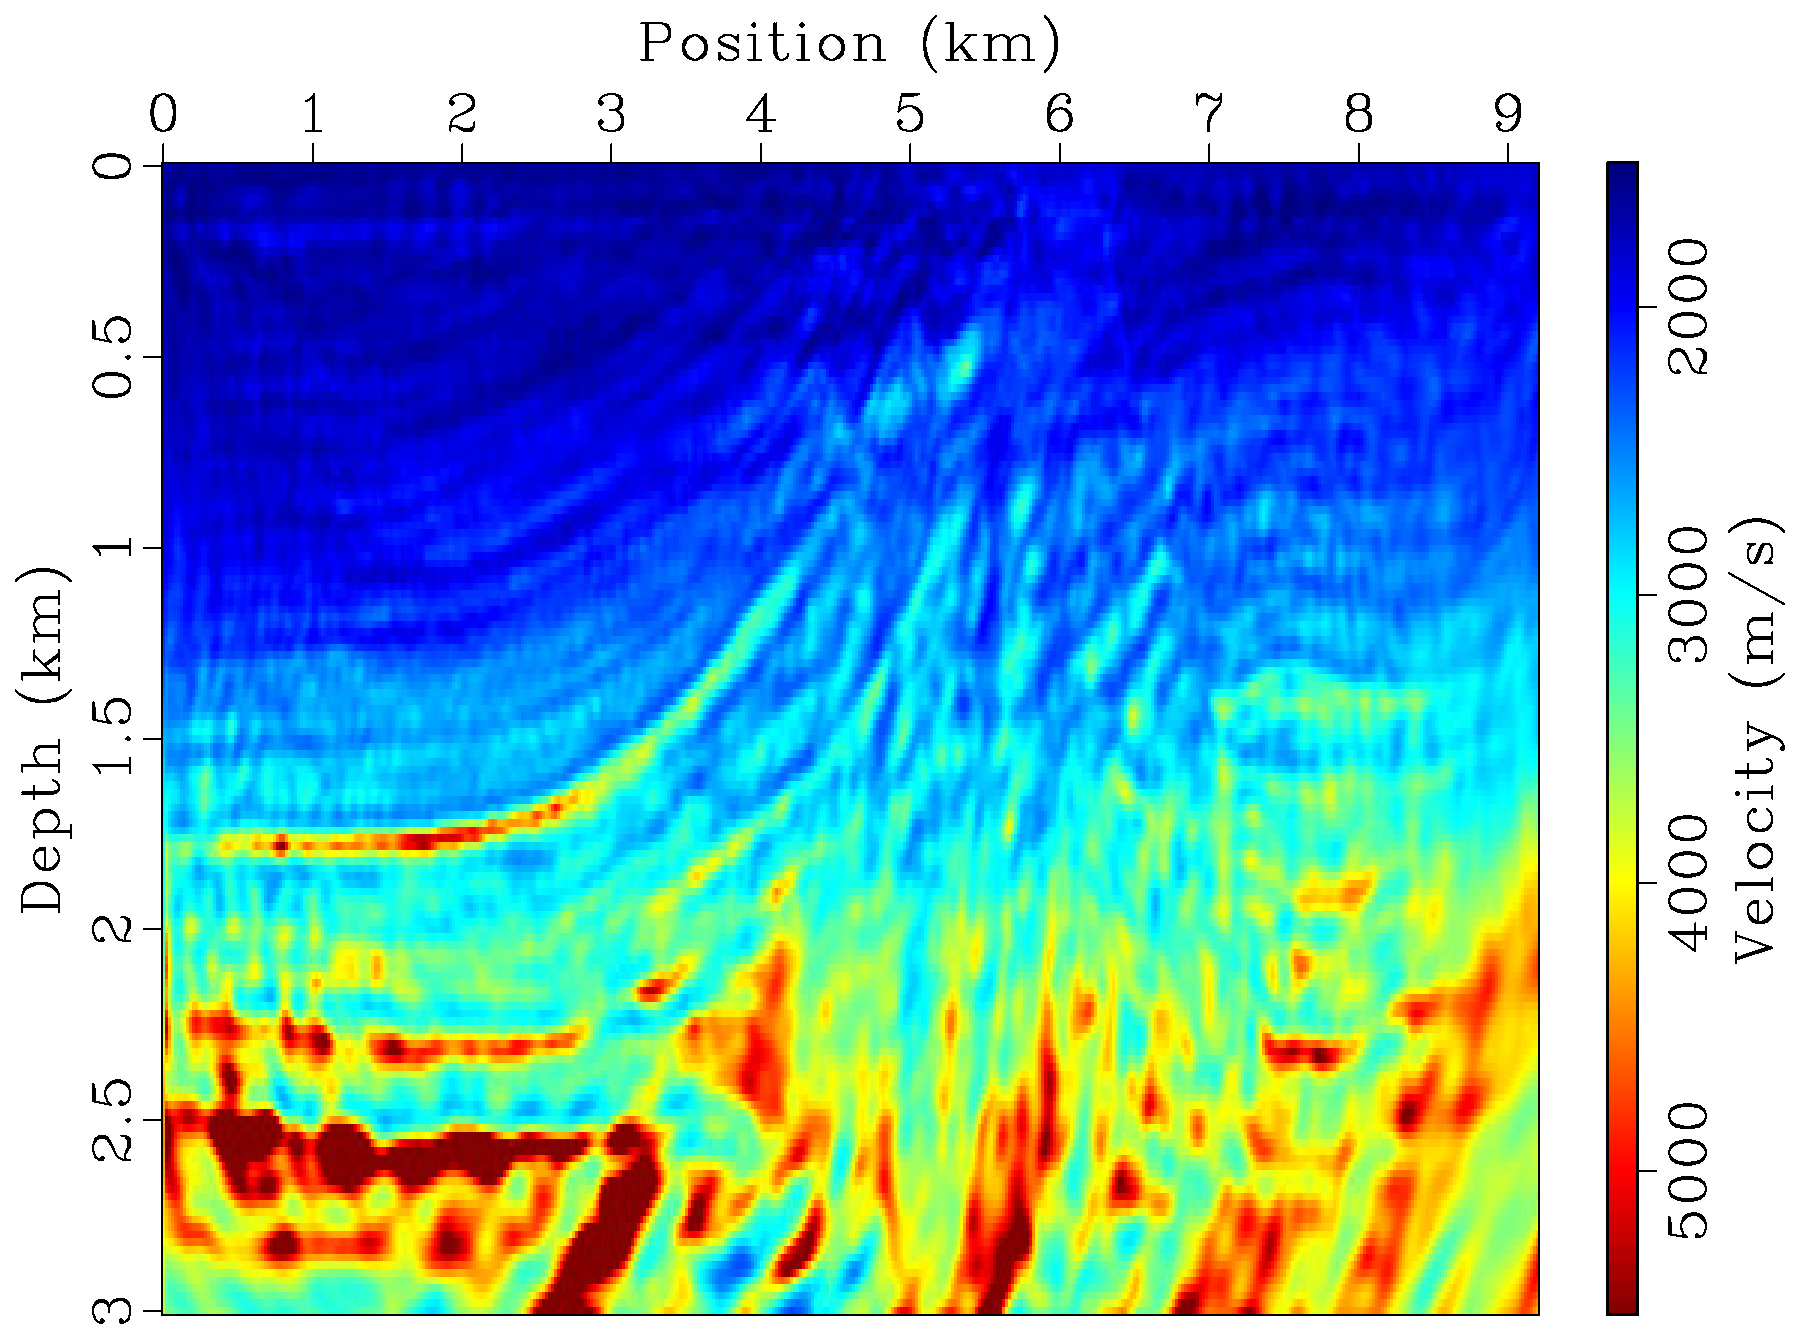
\includegraphics[height=2.1in]{fwi.pdf}
        \caption{无噪音全波形反演结果。}
        \label{fig:无噪音全波形反演结果}
    \end{subfigure}%
    ~
    \begin{subfigure}[b]{0.5\textwidth}
        \centering
        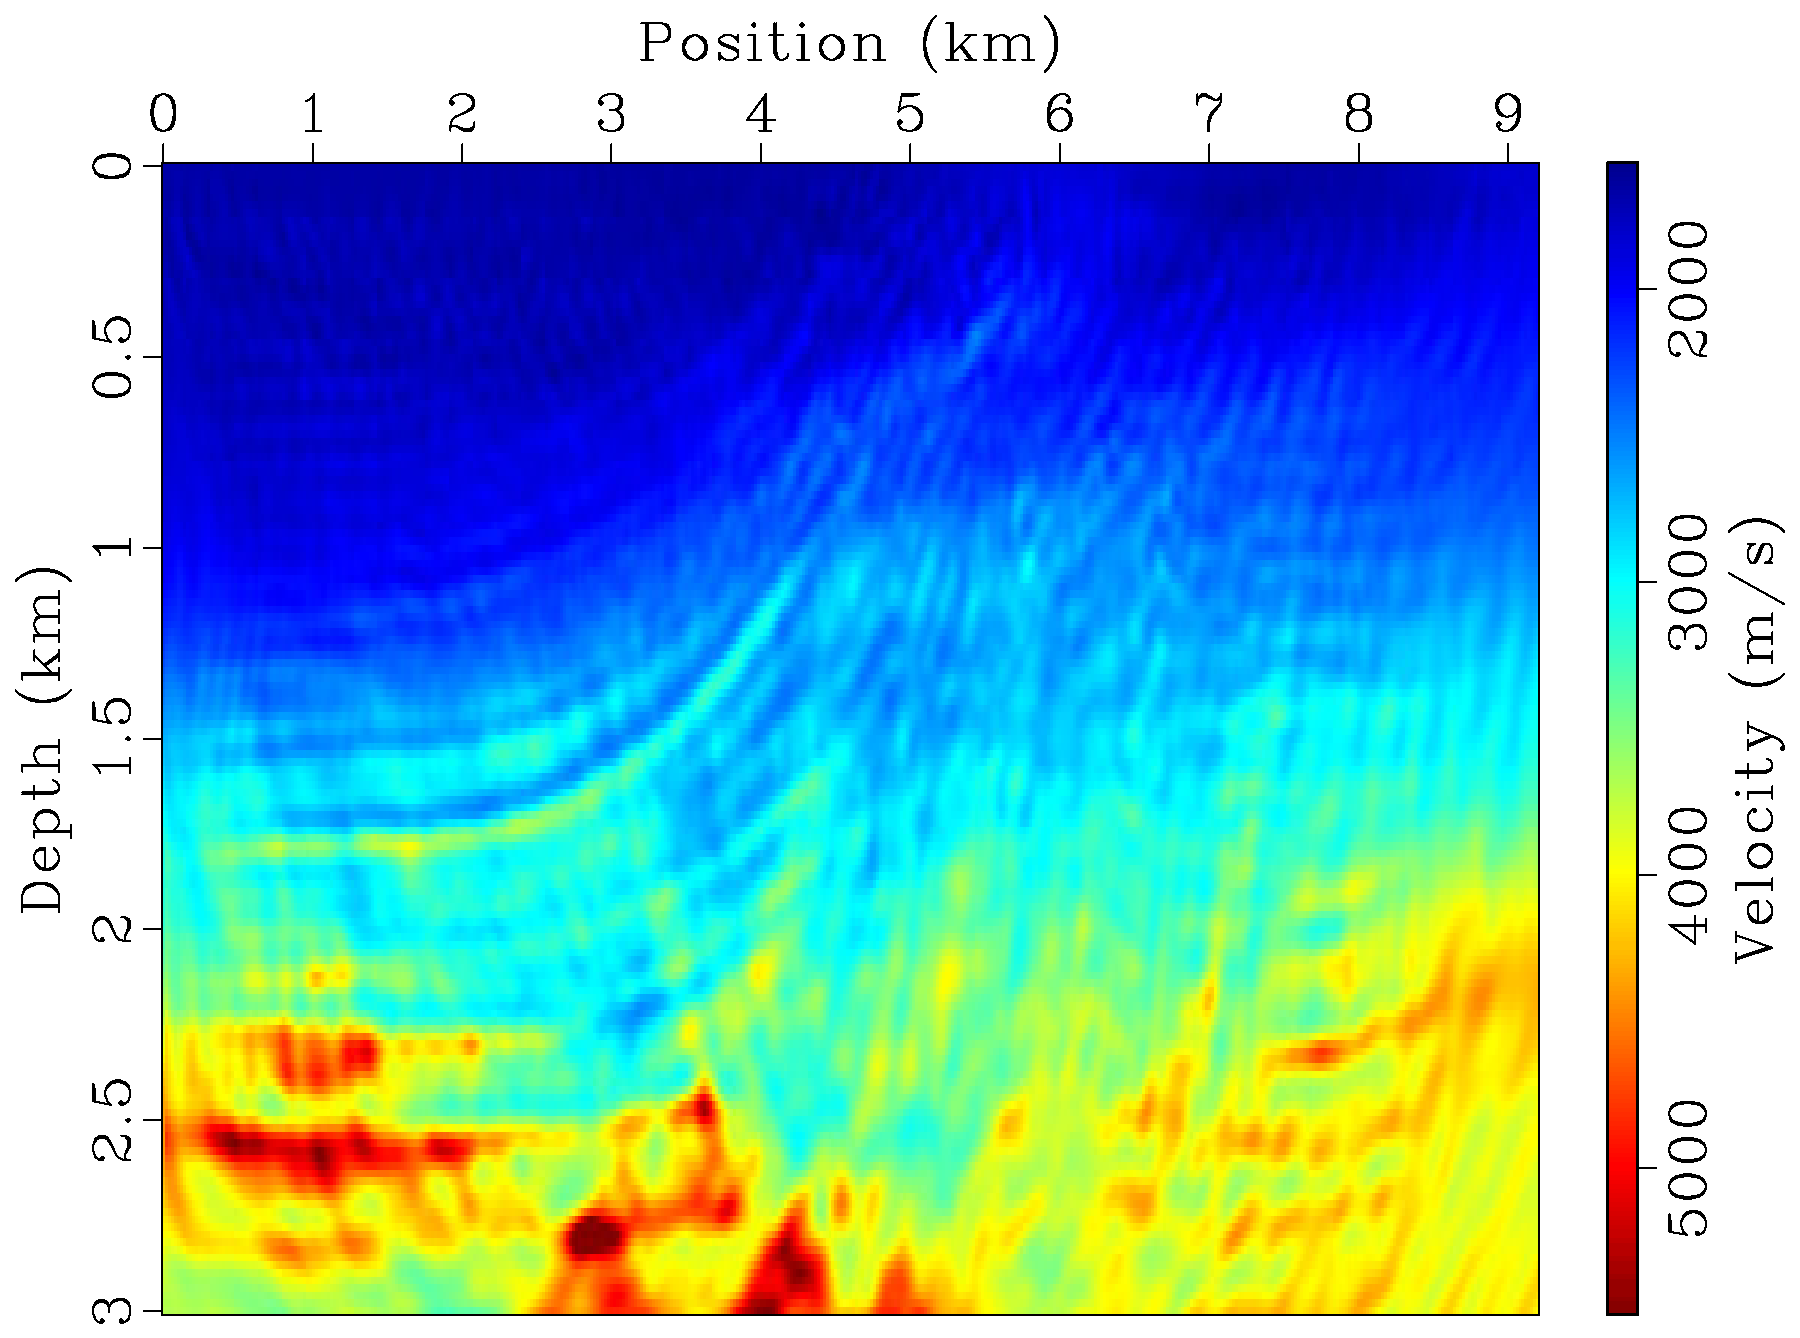
\includegraphics[height=2.1in]{fwi-noise.pdf}
        \caption{有噪音全波形反演结果。}
        \label{fig:有噪音全波形反演结果}
    \end{subfigure}
    \caption{传统全波形反演在无噪音和有噪音情况下的反演成像结果。}
\end{figure}

\begin{figure}[ht]
    \begin{subfigure}[b]{0.5\textwidth}
        \centering
        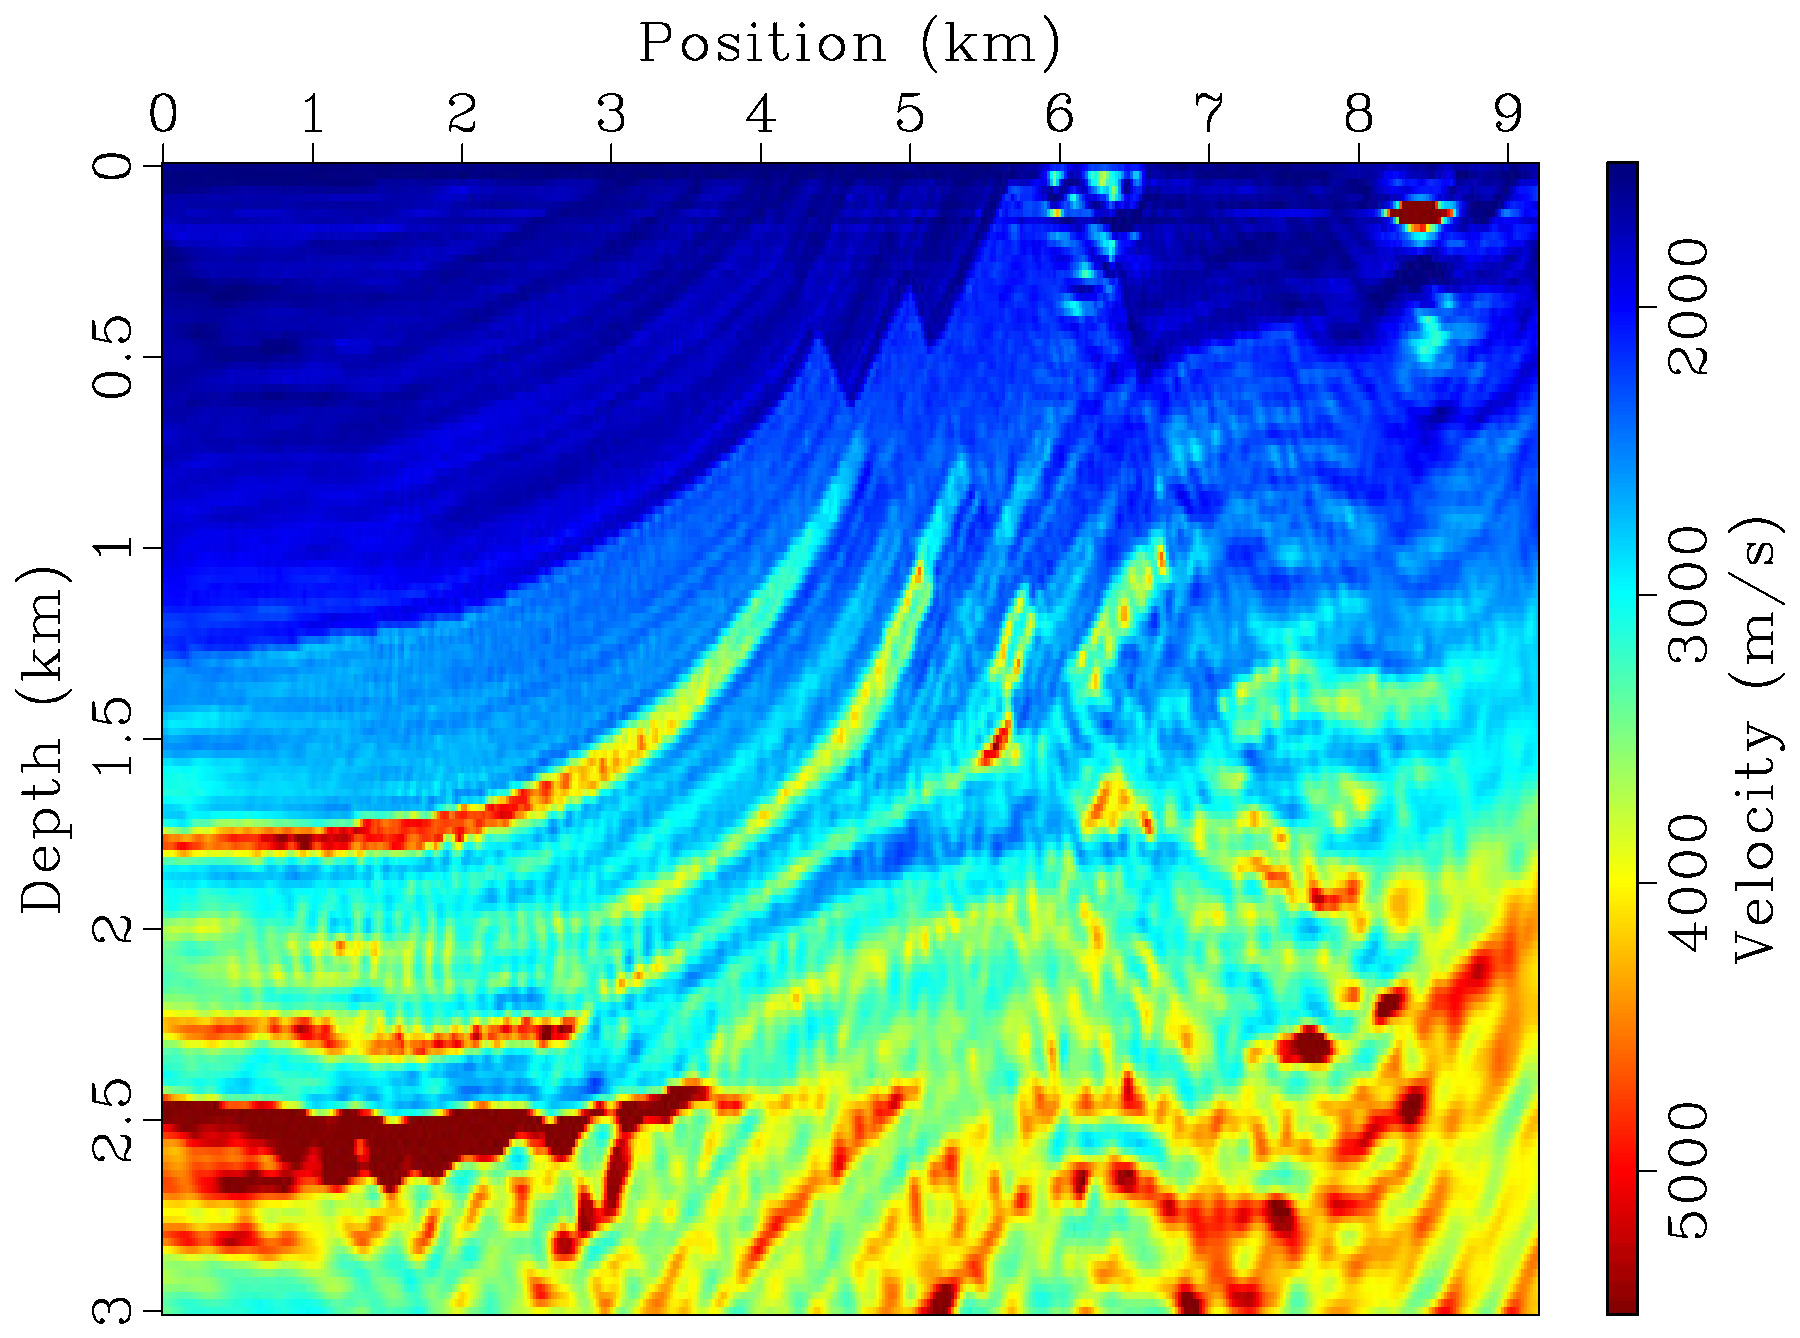
\includegraphics[height=2.1in]{esfwi.pdf}
        \caption{无噪音震源编码全波形反演结果。}
        \label{fig:无噪音震源编码全波形反演结果}
    \end{subfigure}%
    ~
    \begin{subfigure}[b]{0.5\textwidth}
        \centering
        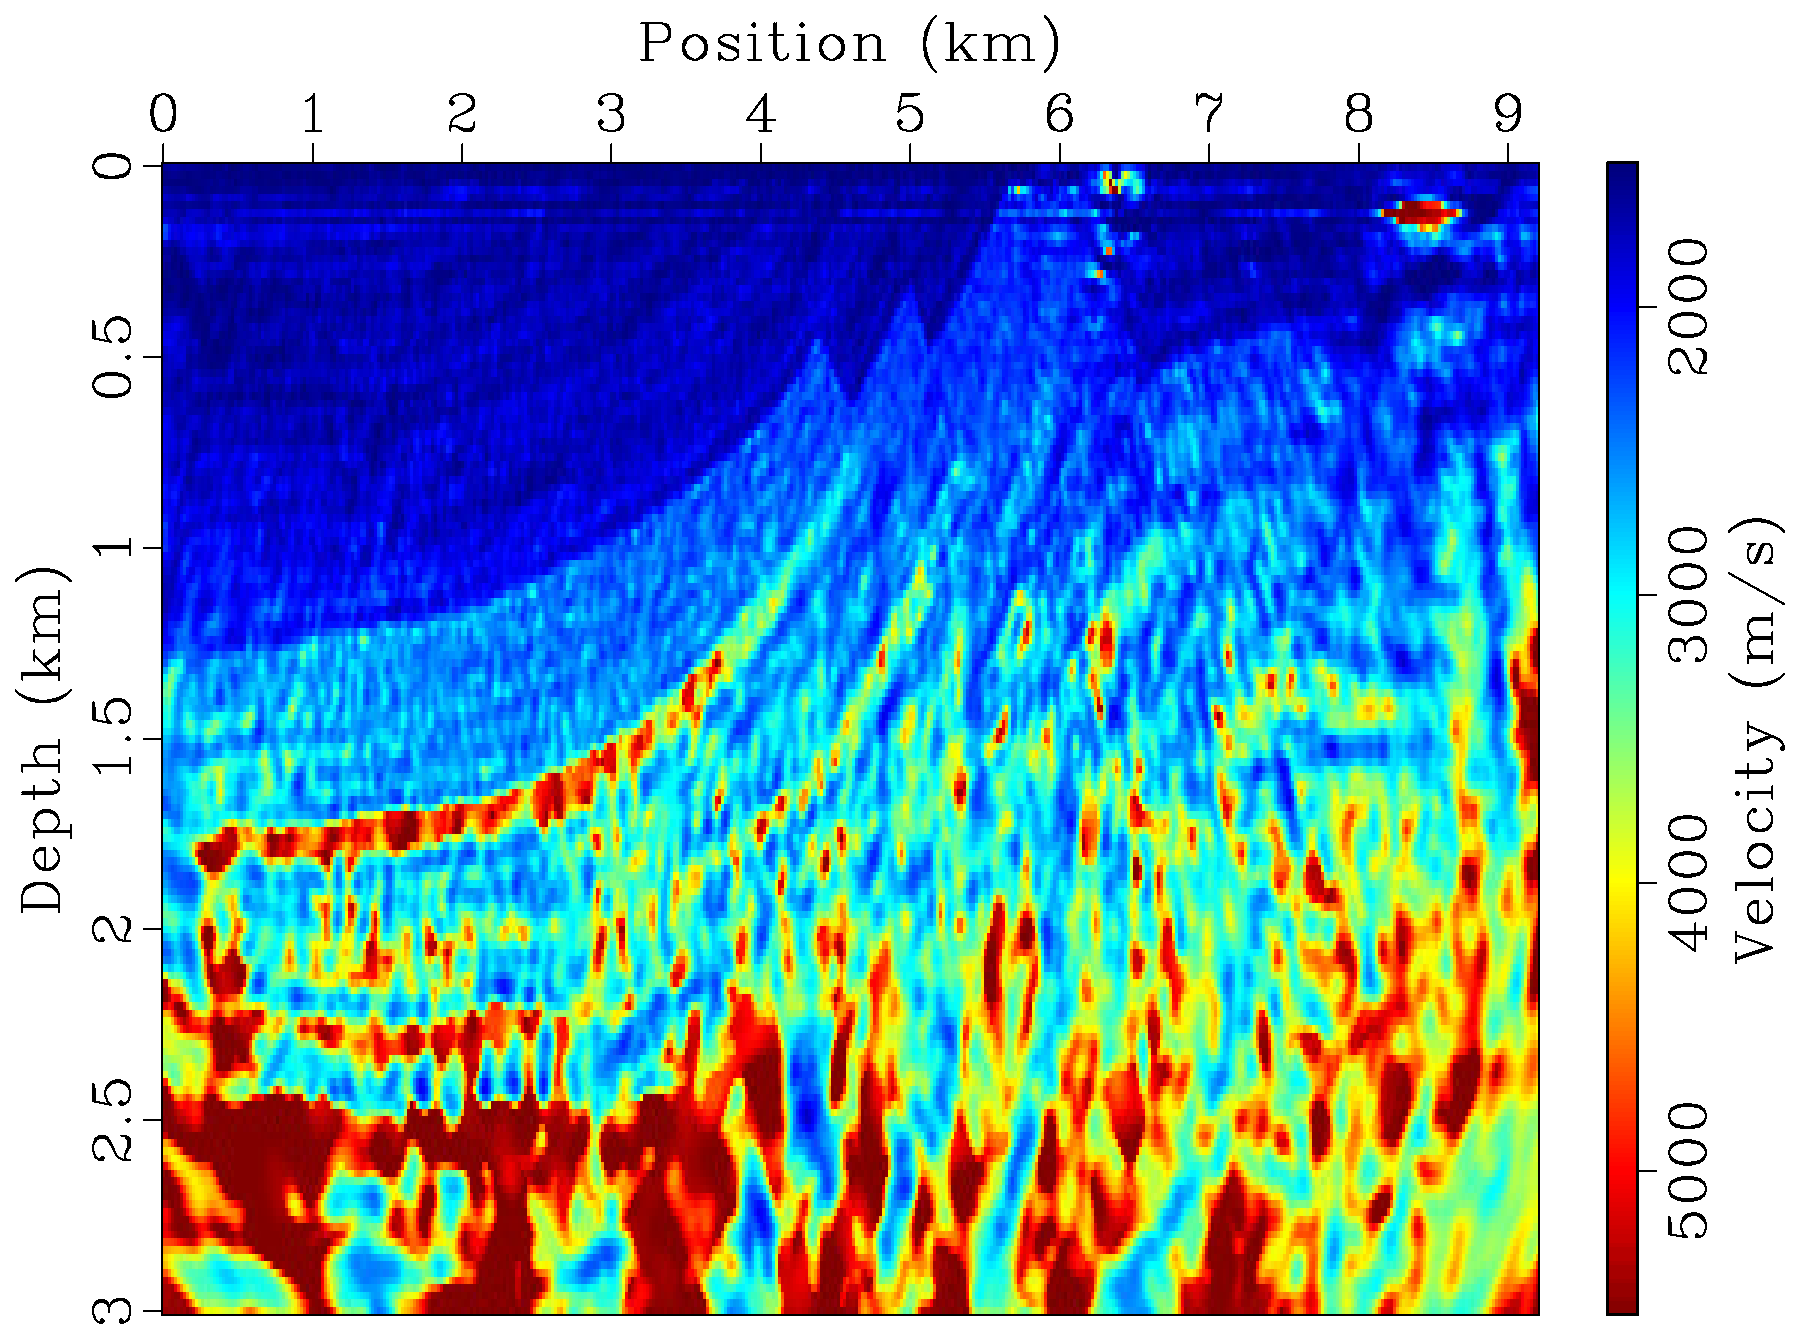
\includegraphics[height=2.1in]{esfwi-noise.pdf}
        \caption{有噪音震源编码全波形反演结果。}
        \label{fig:有噪音震源编码全波形反演结果}
    \end{subfigure}
    \caption{震源编码全波形反演在无噪音和有噪音情况下的反演成像结果。}
\end{figure}

\begin{figure}[ht]
    \begin{subfigure}[b]{0.5\textwidth}
        \centering
        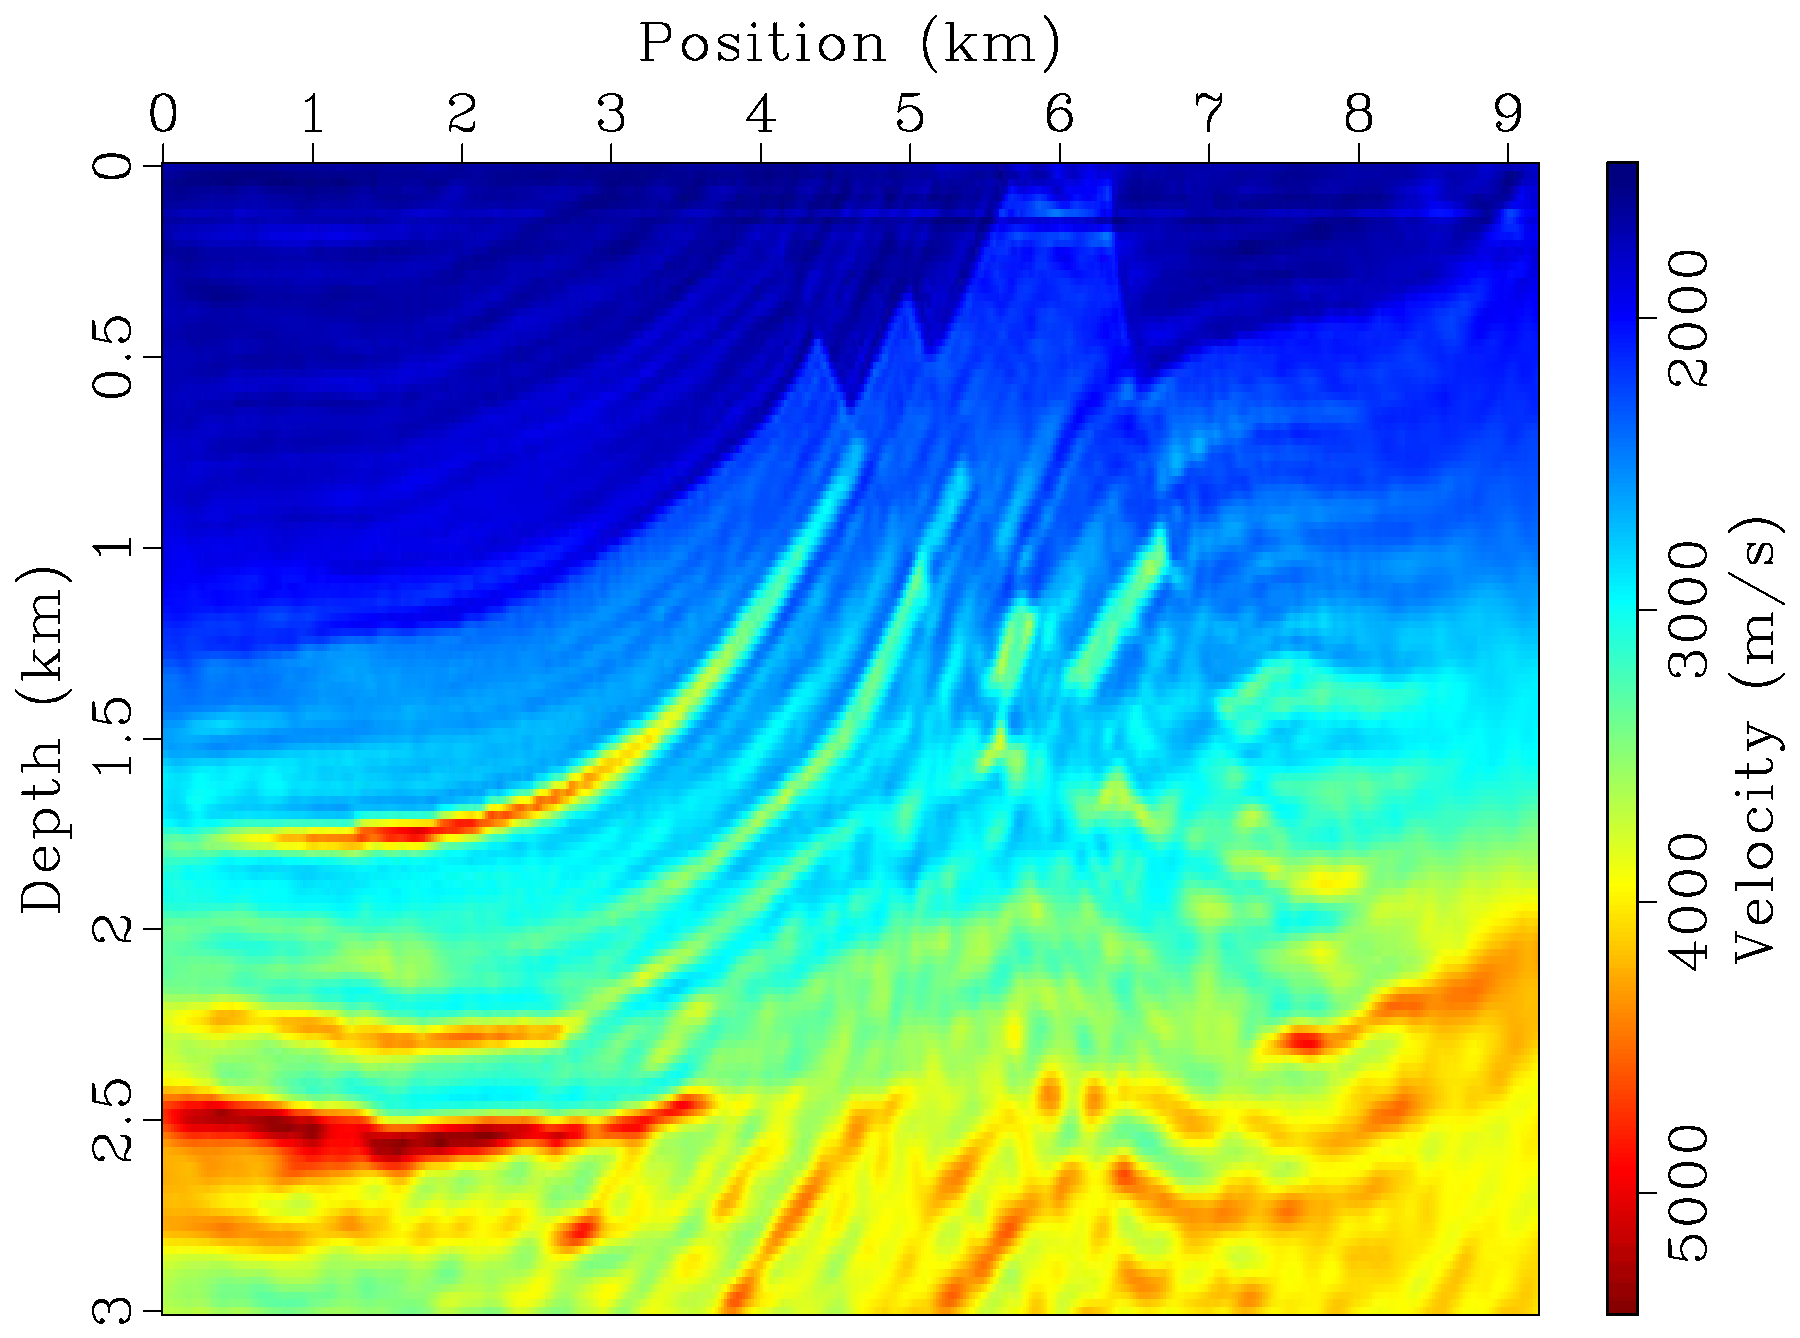
\includegraphics[height=2.1in]{enfwi.pdf}
        \caption{无噪音集合全波形反演结果。}
        \label{fig:无噪音集合全波形反演结果}
    \end{subfigure}%
    ~
    \begin{subfigure}[b]{0.5\textwidth}
        \centering
        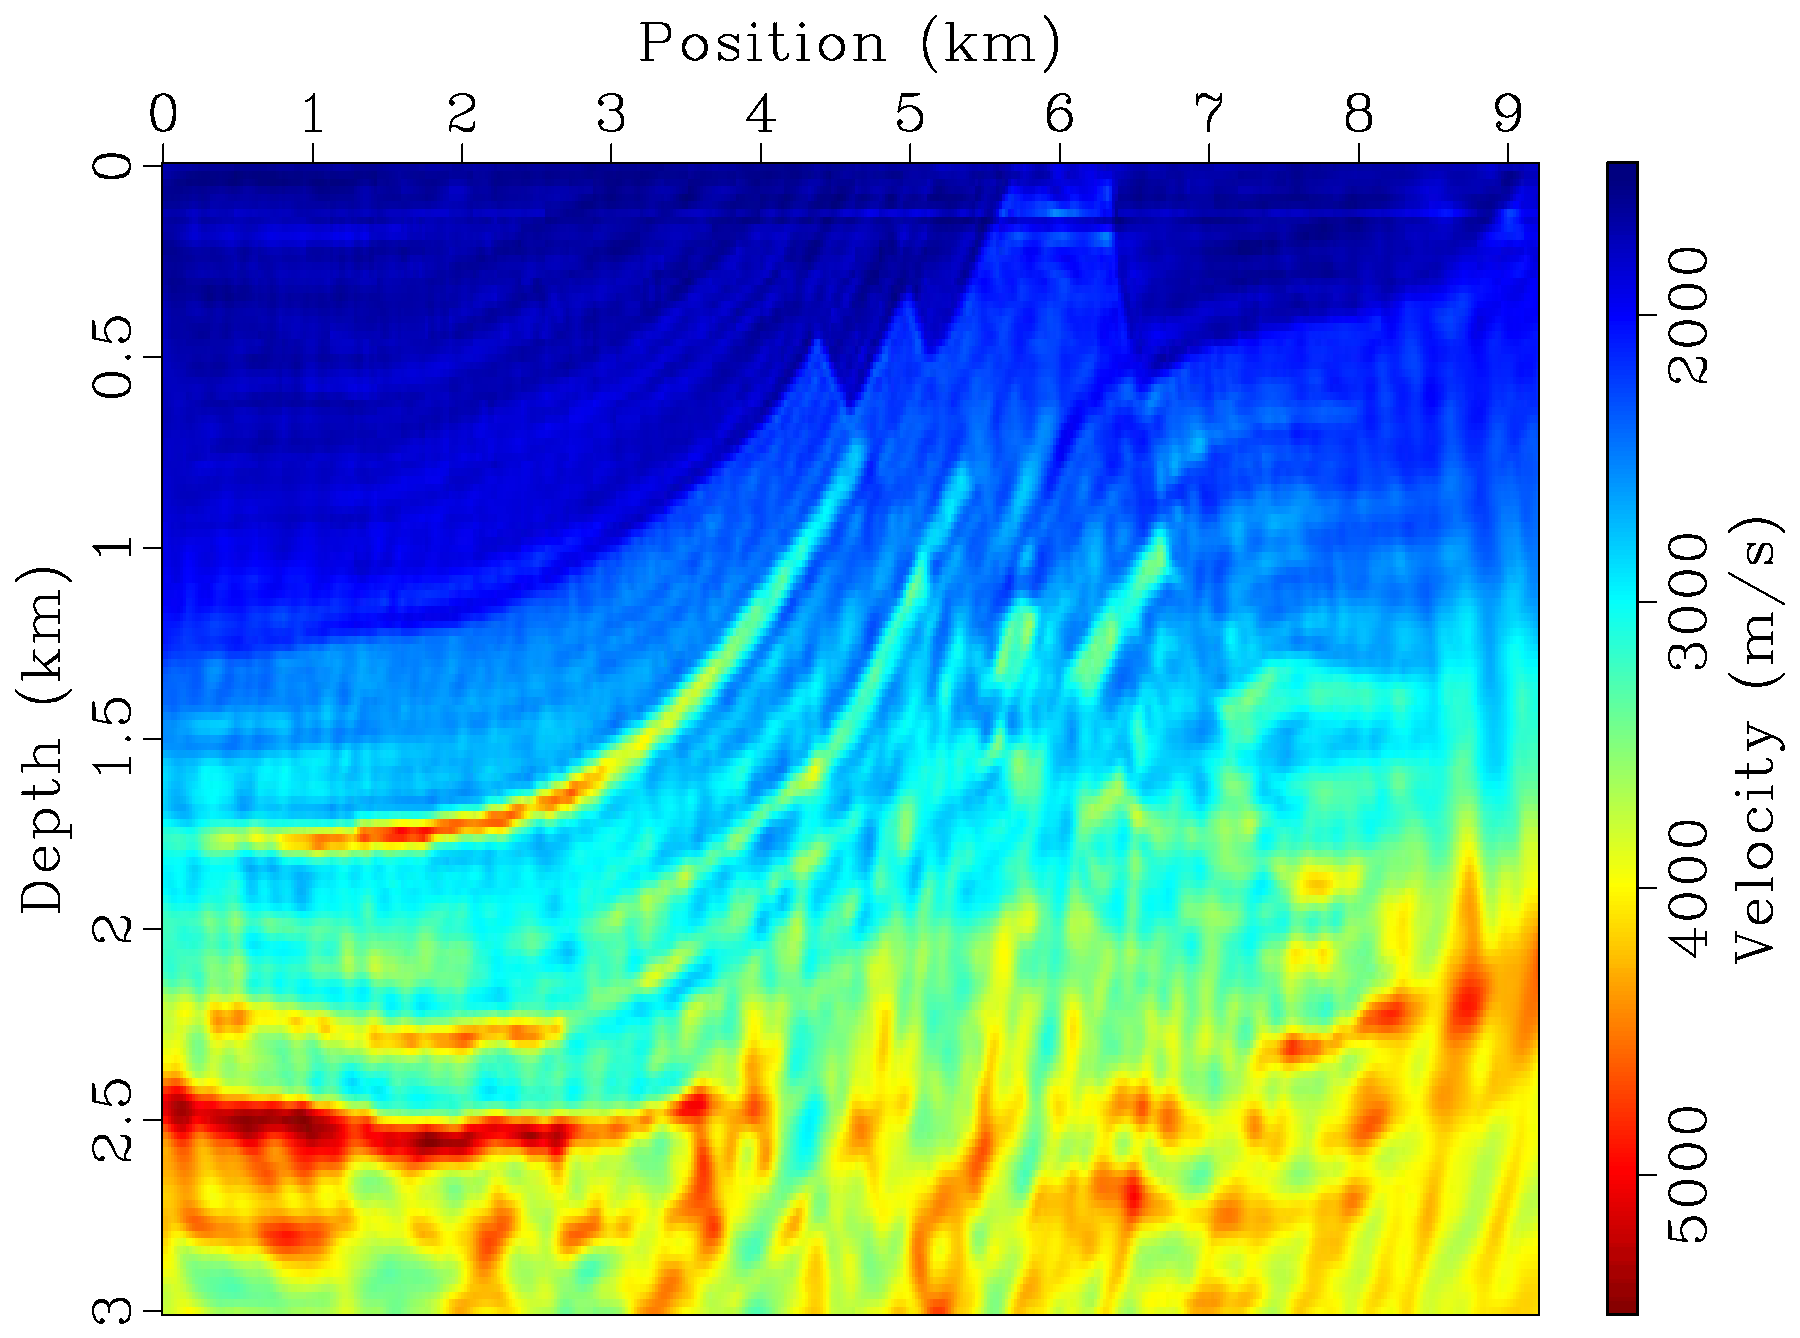
\includegraphics[height=2.1in]{enfwi-noise.pdf}
        \caption{有噪音集合全波形反演结果。}
        \label{fig:有噪音集合全波形反演结果}
    \end{subfigure}
    \caption{集合全波形反演在无噪音和有噪音情况下的反演成像结果。}
\end{figure}

图\ref{fig:无噪音全波形反演结果}、\ref{fig:无噪音震源编码全波形反演结果}、\ref{fig:无噪音集合全波形反演结果}分别描述了无噪音情况下全波形反演、震源编码全波形反演、集合全波形反演算法的成像结果。我们可以看到,在初始模型较差的情况下,传统全波形反演算法只能勾画出大致的速度层状结构,但缺乏高频信息;震源编码全波形反演结果能够反演出较好的层状结构,尤其是在低速区,反演的结果几乎与真实模型相同,但也陷入了局部最优(如图\ref{fig:无噪音震源编码全波形反演结果}右上角红点所示)。集合全波形反演算法克服了全波形反演和震源编码全波形反演算法的不足,清晰的反演出最接近真实的速度模型。在高速区域的反演效果明显好于前两种算法。此外,由于全波形反演算法最终对所有样本基本进行均值化处理,最终反演的速度模型有明显的平滑效果,消除了局部最优的假象。

我们在观测地震记录中加入了幅值为全局地震记录最大值的5\%的白噪音。在较差的初始速度模型和数据噪音的双重影响下,图\ref{fig:有噪音全波形反演结果}、\ref{fig:有噪音震源编码全波形反演结果}、\ref{fig:有噪音集合全波形反演结果}分别描述了无噪音情况下全波形反演、震源编码全波形反演、集合全波形反演算法的成像结果。我们可以看到,在有噪音情况下,三种方法的成像效果都不理想。传统的全波形反演算法几乎无法勾勒出Marmousi模型的大致结构,只有少量的有效信息。震源编码全波形反演算法对数据噪音最敏感,出现了大量的人工假象。而集合全波形反演较有效地克服了数据噪音,在低速区反演出精确的模型,在高速区也较好的对抗了噪音造成的影响。

由此可见,集合全波形算法与传统全波形反演、震源编码全波形反演具有更大的收敛域,且对数据噪音更不敏感。在处理的地震成像中具有更大的应用潜力。

% section 实验结果与分析 (end)

\section{本章小结} % (fold)
\label{sec:本章小结}

本章主要介绍了面向太湖之光超算系统的人工地震成像算法——集合全波形反演方法。本章首先提出了集合全波形反演方法,该方法在可接受的计算效率下,比传统全波形反演方法和基于震源编码的全波形反演方法具有更大的收敛域和更低的噪音敏感度。然后本章对集合全波形整体算法以及核心的集合卡尔曼滤波分析步和地震波波场更新等模块进行计算分析,并针对太湖之光超算系统提出设计与优化思路。紧接着,本章详细阐述了集合全波形反演方法在神威超算系统中的多级优化方案,包括基于集合样本的多层级并行任务分解、面向stencil运算的LDM高效数据复用、随机边界条件以及其他优化方法。随后,本章综合运用上述方法实现并优化了面向神威超算系统并行集合全波形反演算法,充分发挥了神威超算系统的各项资源优势,取得了令人振奋的性能结果。最后,本章在Marmousi模型上进行了数值实验模拟,将集合全波形反演算法与传统全波形反演方法和基于震源编码的全波形反演方法进行比较,验证了集合全波形反演方法具有更大的收敛域和更低的噪音敏感度。

% section 本章小结 (end)